\let\negmedspace\undefined
\let\negthickspace\undefined
\documentclass[journal]{IEEEtran}
\usepackage[a5paper, margin=10mm, onecolumn]{geometry}
%\usepackage{lmodern} % Ensure lmodern is loaded for pdflatex
\usepackage{tfrupee} % Include tfrupee package

\setlength{\headheight}{1cm} % Set the height of the header box
\setlength{\headsep}{0mm}     % Set the distance between the header box and the top of the text

\usepackage{gvv-book}
\usepackage{gvv}
\usepackage{cite}
\usepackage{amsmath,amssymb,amsfonts,amsthm}
\usepackage{algorithmic}
\usepackage{graphicx}
\usepackage{textcomp}
\usepackage{xcolor}
\usepackage{txfonts}
\usepackage{listings}
\usepackage{enumitem}
\usepackage{mathtools}
\usepackage{gensymb}
\usepackage{comment}
\usepackage[breaklinks=true]{hyperref}
\usepackage{tkz-euclide} 
\usepackage{listings}
% \usepackage{gvv}                                        
\def\inputGnumericTable{}                                 
\usepackage[latin1]{inputenc}                                
\usepackage{color}                                            
\usepackage{array}                                            
\usepackage{longtable}                                       
\usepackage{calc}                                             
\usepackage{multirow}                                         
\usepackage{hhline}                                           
\usepackage{ifthen}                                           
\usepackage{lscape}
\usepackage{multicol}

% Marks the beginning of the document
\begin{document}
\bibliographystyle{IEEEtran}
\vspace{3cm}

\title{10.4.ex.13.1}
\author{EE24BTECH11018 - Durgi Swaraj Sharma}

% \maketitle
% \newpage
% \bigskip
{\let\newpage\relax\maketitle}
\renewcommand{\thefigure}{\theenumi}
\renewcommand{\thetable}{\theenumi}
\setlength{\intextsep}{10pt}
\numberwithin{equation}{enumi}
\numberwithin{figure}{enumi}
\renewcommand{\thetable}{\theenumi}
\textbf{Problem:} Find the roots of the following quadratic equations, if they exist, using the quadratic formula:
\brak{i} $3x^2-5x+2=0$\\ 
\solution \\
The roots can be found in multiple methods. We will solve the problem using the Newton-Raphson method, as it works well for our case due to simplicity.\\ 
\textbf{Newton-Raphson method:}\\
From a starting value $x_0$, we iterate as following:
\begin{align}
  x_{n+1} = x_n - \frac{f\brak{x_n}}{f^{\prime}\brak{x_n}}
\end{align}
If the roots are real, $x_n$ will converge to a root; but if the roots are complex and the coefficients are real, $x_n$ will converge either to an extrema or grow boundlessly if our inital guess is not complex. \\In our case,
\begin{align*}
  f\brak{x} &= 3x^2-5x+2\\
  f^{\prime}\brak{x} &= 6x-5
\end{align*}
And the update equation will be
\begin{align}
  x_{n+1} = x_n - \frac{3x^2-5x+2}{6x-5}
\end{align}
Taking starting values of $x$ as $x = 10, -10$, in 9 iterations each, we find the roots to be $0.666667$ and $1.000000$.
\begin{figure}
  \centering
  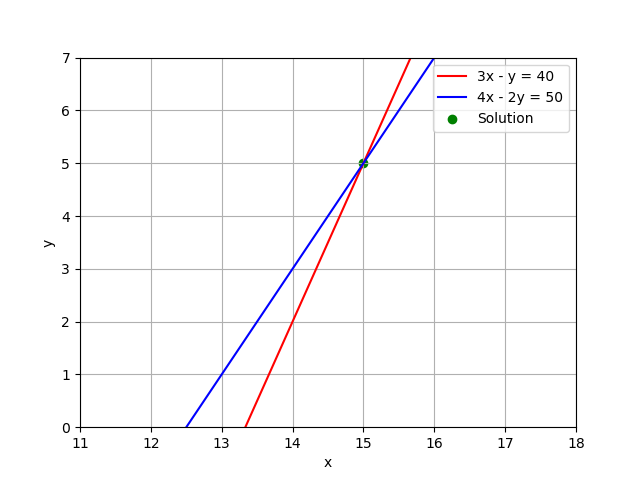
\includegraphics[width=\columnwidth]{/home/gvt1/sdcard/github/EE1003/Assignment4/figs/fig.png}
  \caption{Graphical verification}
\end{figure}
\end{document}
